\documentclass[12pt,journal,compsoc]{IEEEtran}
\usepackage{ae}
\usepackage{lipsum}  
\usepackage{amsmath, amssymb, amsfonts, amsthm}
\usepackage{mathrsfs}
\usepackage{epsfig}
\usepackage{mathtools}
\usepackage{algorithm,algorithmic}
\usepackage{graphicx}
\usepackage{comment}
\usepackage{array}
\usepackage{verbatim}
\usepackage{amsfonts}
\usepackage{amssymb}
\usepackage{float}
\usepackage{pgfplots}
\usepackage{graphics}
\usepackage[utf8]{inputenc}
\usepackage[normalem]{ulem}
\usepackage{multicol}
\usepackage{booktabs}
\usepackage{mathrsfs}
\usepackage{subfig}
\usepackage{subcaption} 
\usepackage[english]{babel}
\usepackage[pdftex]{hyperref}
\usepackage{ragged2e}
\usepackage{indentfirst}


\begin{document}

\title{Making Good Movie Recommendations for Users}

\author{Zihe Wang (zw2624), Di Ye (dy2404)\\ Ziyao Zhang (zz2583), Yinhe Lu (yl4372)}
% \author{Di Ye, Zihe A, Ziyao Zhang, Yinhe Lu}
\markboth{Data Science Institute, Columbia University}%
{Shell \MakeLowercase{\textit{et al.}}: Bare Demo of IEEEtran.cls for Computer Society Journals}

\IEEEcompsoctitleabstractindextext{%

\selectlanguage{english}

\begin{abstract}
\justify
Our business objective is to recommend movies to users, and we choose those users who have already watched at least a few movies on the platform. We want to make sure that users are interested in the movies recommended by our algorithm. We explore three methods of building a recommendation system to suggest movies to users. We tried with two brute-force collaborative filtering algorithms to recommend movies to users and compared their results to a baseline model.
\begin{itemize}
    \item Neighborhood-Based Collaborative Filtering: Item-Based Model
    \item Model-based Collaborative Filtering: Matrix Factorization
\end{itemize}
We predicted a user’s unknown ratings by using the similarities in conjunction with the user’s known rating to initialize the item-based k-Nearest Neighbors and conduct matrix factorization. We later discussed our empirical results by setting up cross-validation and evaluating the accuracy on training and testing dataset. 


\end{abstract}

\keywords{Recommendation System, Collaborative Filtering}
}

\maketitle

\IEEEpeerreviewmaketitle

\section{Introduction}
Recommendation systems, first introduced in 1992, have been prevalent in dealing with massive information by suggesting relevant items or products to users. As internet has been developing so rapidly, recommendation systems have become an efficient way to extract useful and relevant information from users and then generate useful suggested items to users according to their explicit and implicit feedback.

Collaborative filtering (CF), which refers to the use of rating from multiple users in a collaborative way to predict missing ratings, becomes one of the most popular and efficient techniques for movie recommendation systems. Two important classes of collaborative filtering techniques: memory-based/neighborhood-based and model-based collaborative filtering have been used and evaluated in our project. 

\subsection{Objective}

Our recommendation system is to help users connect to the movies they love. It can predict whether a certain user would enjoy a movie based on how they rated other movies. From there, we can generalize personal movie recommendation for each user based on their unique taste. Movie recommendation system is essential for online media-service provider companies such as Netflix and Hulu. The success of a movie recommendation system will make a big difference to existing/potential customers and the companies' business. 

A basic acceptance criteria we need to define is that how well is our recommendation system, which means whether a user will favor the movie that our system recommend to them. To measure this criteria, first, we need to make sure our recommendation system is better than the baseline and produce a decent coverage score. In order to achieve this, we need to tackle two main objectives: predict the ratings that a user would give to a movie that he/she has not yet rated, then minimize the difference between the predicted ratings and actual ratings(using $RMSE$ and $MAE$).

We tried to build models that predict the unknown rating of users to movies according to their previous ratings and recommend top-k movies to the users. Then we evaluated the performance of our model and compared it to a baseline model.

\subsection{Data}

In our project, we used the dataset from MovieLens to build a recommendation system to recommend movies to users. The dataset (ml-20m) describes 5-star rating and free-text tagging activity from [MovieLens](http://movielens.org), a movie recommendation service. It contains 20000263 ratings and 465564 tag applications across 27278 movies. These data were created by 138493 users between January 09, 1995 and March 31, 2015. This dataset was generated on March 31, 2015, and updated on October 17, 2016. No demographic information is included. Each user and movie are represented by their corresponding id, and no other information is provided.

\section{Data Preparation and Exploration}
% \subsection{Data Visualization and Subsampling}
First, since we need to subsample the dataset, we plot the distribution of ratings. We can see that ratings exhibit a long-tail property(Figure1), which can heavily influence the results by the ratings on the popular items. In our sampling techniques, we try to preserve this distribution of number of ratings. Hence, first by checking the proportion of the number of ratings in the total number of ratings in different ranges, we subsampled the dataset by preserving these proportions. We chose rating records in a random manner. 

Figure2 and Figure3 showed the distribution of ratings after subsampling, we can see that the original distribution has been preserved. After subsampling, we have 9998 users and 3000 movies in total. All selected users have rated at least 8 movies. Each movie has been rated at least 21 times. 

\begin{figure}[H]
\centering
\caption{The long tail of rating frequencies}
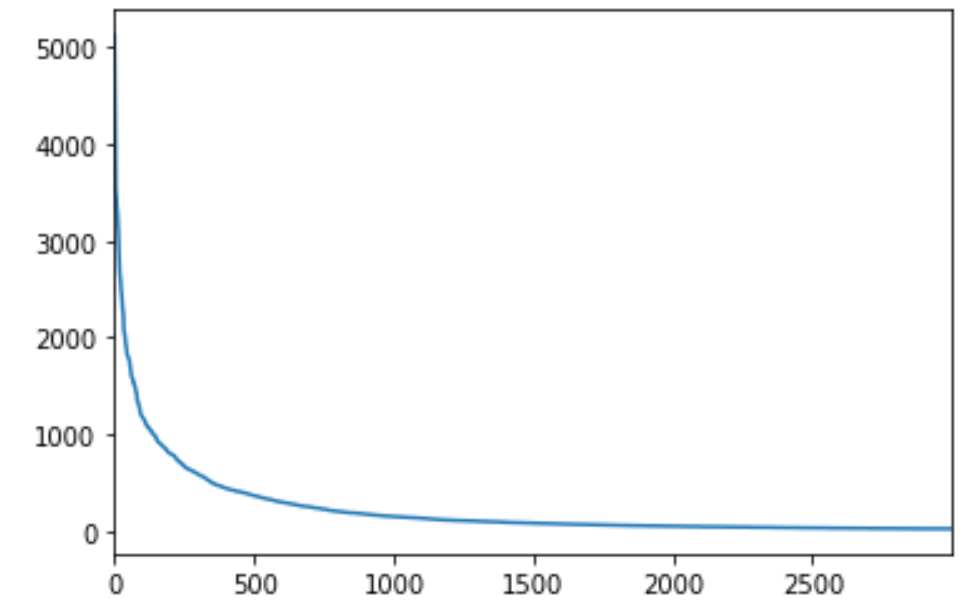
\includegraphics[width=0.30\textwidth]{img/longtail.png}
\label{fig_sim}
\end{figure}

\begin{figure}[H]
\centering
\caption{User Rating Frequencies after Subsampling}
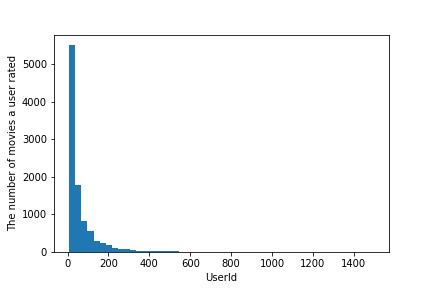
\includegraphics[width=0.30\textwidth]{img/User.jpg}
\label{fig_sim}
\end{figure}

\begin{figure}[H]
\centering
\caption{movie Rating Frequencies after Subsampling}
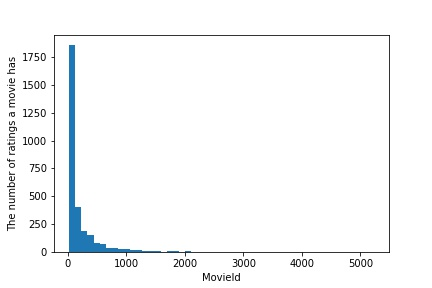
\includegraphics[width=0.30\textwidth]{img/movie.jpg}
\label{fig_sim}
\end{figure}

\section{Methods}

\subsection{Baseline Model}
We use a baseline model for comparing results. The model uses the baseline estimate for given user and item. \footnote{https://surprise.readthedocs.io/en/stable/basic\_algorithms.html}

$$\hat \mu_i = b_{ui} = \mu + b_u + b_i$$
If user $u$ is unknown, then the bias $b_u$ is assumed to be zero. 
% The prediction $\hat r_{ui}$ is generated from a normal distribution $N(\hat \mu,\hat \sigma^2)$ where $\hat \mu$ and $\hat \sigma$ are estimated from the training data using Maximum Likelihood Estimation:

% $$\hat \mu = \frac{1}{|R_{train}|}\sum_{r_{ui} \in R_{train}}r_{ui}$$
% $$\hat \sigma = \sqrt{\sum_{r_{ui} \in R_{train}} \frac{(r_{ui} - \hat \mu) ^ 2}{|R_{train}|}}$$

\subsection{Collaborative Filtering}

\subsubsection{Neighborhood-Based CF: Item-Based Model}

We used a neighborhood-based method to predict the rating of specific user-item combinations. For this dataset, we implemented an Item-based model. Item-based Neighborhood models allow for natural explanations to the user. Item-based methods can be more stable than user-based methods, since there is likely more overlap between items than users. An extra item is added less frequently than users to total dataset, so it could be less computational expensive.
For Item-based Neighborhood Models, similarities need to be computed between items. Three similarity function variants are tried in our project: Cosine, Pearson baseline, Pearson. 

{\bf RawCosine}($i, j$) = $$\frac{\sum_{k \in I_u \cap I_v} r_{uk} r_{vk}}{\sqrt{\sum_{k \in I_u \cap I_v}r_{uk}^2} \sqrt{\sum_{k \in I_u \cap I_v}r_{vk}^2}}$$

{\bf PearsonBaseline}($u, v$) = $$\frac{\sum_{k \in I_u \cap I_v} (r_{uk} - b_{uk})(r_{vk}-b_{vk})}{\sqrt{\sum_{k \in I_u \cap I_v}(r_{uk} - b_{uk})^2} \sqrt{\sum_{k \in I_u \cap I_v}(r_{vk} - b_{vk})^2}}$$

{\bf Pearson}($u, v$) = $$\frac{\sum_{k \in I_u \cap I_v} (r_{uk} - \mu_u)(r_{vk}-\mu_v)}{\sqrt{\sum_{k \in I_u \cap I_v}(r_{uk} - \mu_u)^2} \sqrt{\sum_{k \in I_u \cap I_v}(r_{vk} - \mu_v)^2}}$$

The predicted rating $\hat r_{uj}$ of user $u$ for target item $t$ is as follows:
$$\hat r_{uj} = \mu_u + \frac{\sum_{v \in P_u(j)} Sim(u,v) (r_{vj} - \mu_v)}{\sum_{v \in P_u(j)} |Sim(u, v)|}$$

where $P_u(j)$ is the peer set of $k$ closest neighbors to user $u$ that have a rating for item $j$.

The cosine function applied on the raw ratings to calculate the similarity. In general, the Pearson is preferable to the cosine because it adjusts the bias effect of mean-centering. 

\subsubsection{Model-based CF: Non-negative Matrix Factorization}
Non-negative matrix factorization (NMF) has a high level of interpretability in understanding the user-item interactions. The optimization formulation in NMF is shown below:
$$Minimize J = \frac{1}{2}||R-Q^TP||^2$$ with  $$P_i, Q_i \ge 0$$ 
at each iteration, the matrices are updated:
$$p_{uf} \leftarrow p_{uf} \cdot \frac{\sum_{i \in I_u} q_{if}
\cdot r_{ui}}{\sum_{i \in I_u} q_{if} \cdot \hat{r_{ui}} +
\lambda_u |I_u| p_{uf}}$$\\
$$q_{if} \leftarrow q_{if} \cdot \frac{\sum_{u \in U_i} p_{uf}
\cdot r_{ui}}{\sum_{u \in U_i} p_{uf} \cdot \hat{r_{ui}} +
\lambda_i |U_i| q_{if}}$$\\

We used the following parameter to adjust our method:
\begin{itemize}
    \item rank – The number of factors. 
    \item epoch – The number of iteration of the SGD procedure. 
    \item $p_u$ – The regularization term for user factor.
    \item $q_i$ – The regularization term for item factor.
\end{itemize}
\subsection{Evaluation Metrics}

\subsubsection{Cross-Validation}
Cross-validation is a useful technique to evaluate machine learning models on a limited data sample.
Cross-validation is also important for searching best combination of parameters. Since test set should never be exposed to the model before we finalize our model. Therefore, first, we split dataset into train set(80\%) and test set(20\%). Then we perform a 5-fold cross validation on the train set to help us select the best combination of parameters of our model. Finally, we refit the model on the train dataset using the best combination of parameters we got and test on the test set.


\subsubsection{Accuracy Metrics}

Next, we need to determine how good is our model. In our project, we used the root mean squared error ($RMSE$) and the mean absolute error ($MAE$) to be our evaluation metrics.

We define $r_{uj}$ to be the value of the rating of the entry $(u, j)$ for user $u$'s rating on item $j$ in the test set, and $\hat r_{uj}$ be the predicted rating of the entry $(u,j)$.The error is given by $e_{uj} = \hat r_{uj} - r_{uj}$.The set $E$ corresponds to the held out entries in the hold-out methods.
$$RMSE = \frac{\sqrt{sum_{(u,j) \in E}e_{uj}^2}}{|E|}$$
$$MAE = \frac{sum_{(u,j) \in E}|e_{uj}|}{|E|}$$
These two measurements can tell us how well our model predicted ratings. Compared to $MAE$, $RMSE$ is more sensitive to the outliers, and $MAE$ is more robust to them. Also, $MAE$ is easier to interpret than $RMSE$. So we decide to choose both measurements.


\subsubsection{Coverage}

Coverage is the distribution of accuracy over users, items and catalog.
After we got the predicted ratings of the movies in the testset, we sorted the ratings in descending order and recommend top-10 movies to each user. We considered a movie as a good recommendation for that user if the user gives a true rating of 4 or higher to that movie. If the proportion of such movie in the total number of movies that we recommended to a user is greater or equal to 50\%, then we count that user as a well-recommended user. Same logic applied to the standard of a well-recommended item. We used the following equation to calculate user-coverage (UC), item-coverage (IC), and catalog-coverage (CC).

User-coverage is the number of well-recommended users divided by the total number of users.
$$ UC = \frac{\# Well recommended Users}{\# Total Users}$$


Item-coverage is the number of well-recommended items divided by the total number of items.
$$ IC = \frac{\# Well recommended Items}{\# Total Items}$$

Catalog-coverage is the number of union of items that have been recommended to users divided by the total number of items.
$$CC = \frac{|\bigcup_{u=1}^mT_u|}{n}$$
where $T_u$ is the set of top-$10$(at most 10) items recommended to user $u$, and $n$ is total number of items.

\subsection{Hyper-parameter Tuning}

For the neighborhood-based method, we tuned on the number of nearest neighbor $k$ and three similarity measures.

For the model-based method, we tuned on the number of factors and also regularization parameters.

\subsection{Use of Package}

We started with two choices: scikit-surprise and Spark Mlib. We investigated and built model using both packages. We ran a simple Grid Search with cross validation as a trial run and it turned out that they yielded similar results. However, as seen in the figure below, using spark is much more expensive and time-consuming compared to the paralleled SURPRISE package. So, in order to save time and limit cost, we decide to use SURPRISE package, but we attached the implemented spark method in repository. 
\begin{figure}[H]
\centering
\caption{CPU usage on G-cloud: first peak spark, later surprise}
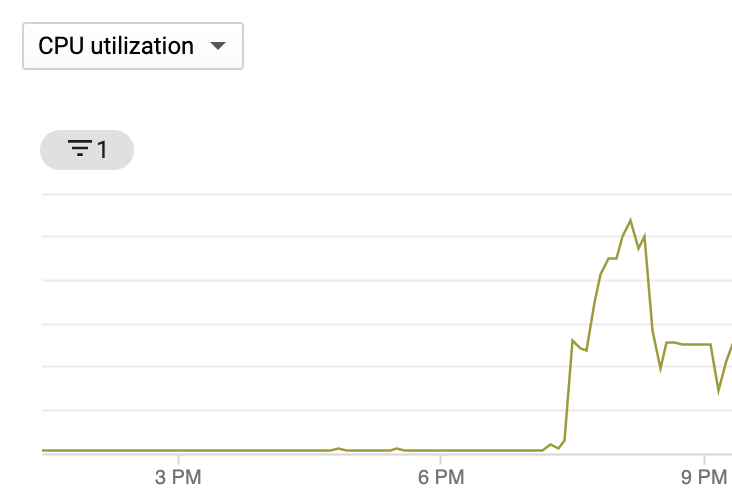
\includegraphics[width=0.30\textwidth]{img/cpu.png}
\label{fig_sim}
\end{figure}



\section{Results}

\subsection{Neighborhood-Based}
For this model, we considered tuning two parameters, the number of neighbors and the similarity equations. First, we tried to use gridsearch and cross-validation to search the best combination of parameters. However, the searching time is too long to take this as a practical approach. So we decided to first use default neighbor size and search the similarity measure, and then search the best neighborhood size. For the similarity equation, we tried with cosine, pearson-baseline, and pearson equations. For the neighborhood size, we tested seven different $k$ values (5, 15, 25, 35, 45, 55, 65). We calculated both $MAE$ and $RMSE$ for each searching epoch, we used $RMSE$ to decide which parameter is the best parameter for the model. First, pearson-baseline is chosen to be the best parameter. Then we got when $k$ = 5, $RMSE$ reach the lowest which is 0.88823, and $MAE$ is 0.68577. We used these two parameter to further evaluate on the test set, and calculate user-coverage, item-coverage, and catalog-coverage. Then we compared the result with the model-based CF and the baseline model.

\begin{figure}[H]
\centering
\caption{RMSE values with different k}
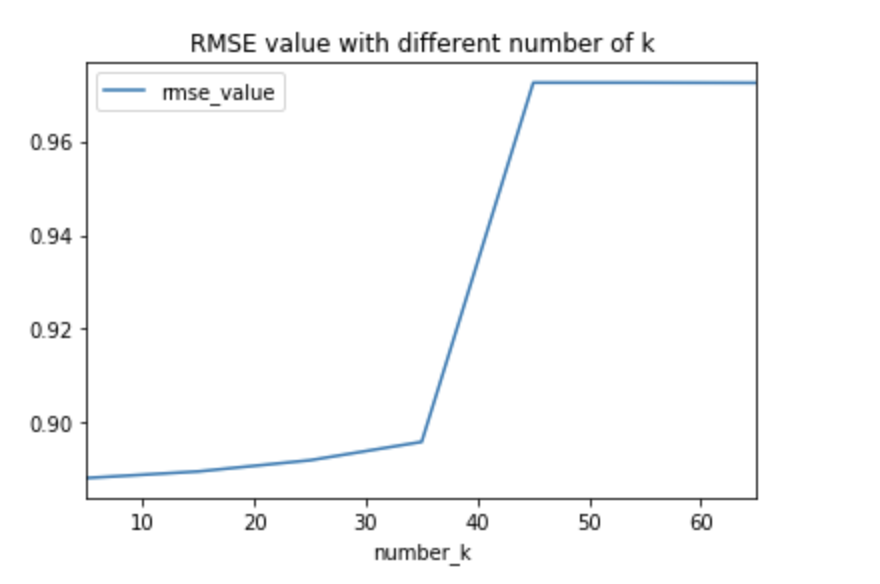
\includegraphics[width=0.30\textwidth]{img/RMSEk.png}
\label{fig_sim}
\end{figure}

\begin{figure}[H]
\centering
\caption{MAE values with different k}
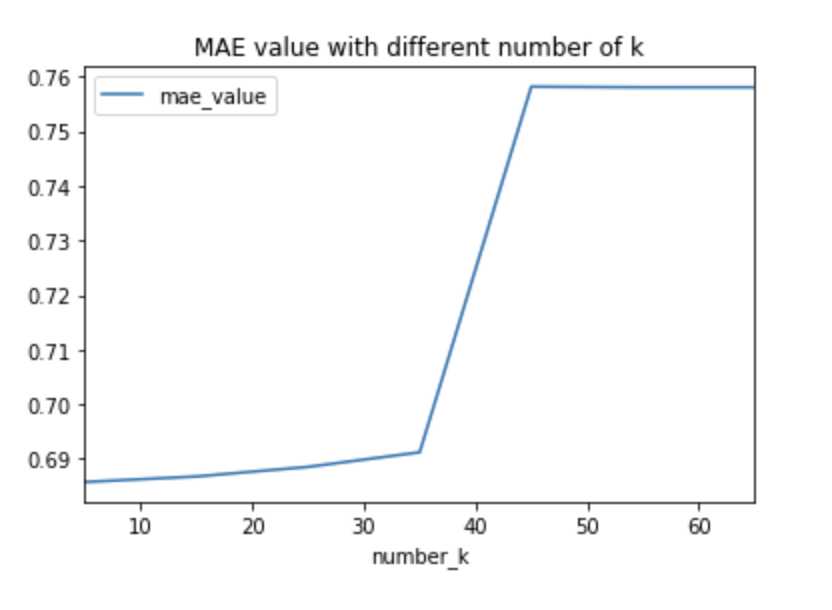
\includegraphics[width=0.30\textwidth]{img/MAEk.png}
\label{fig_sim}
\end{figure}


\begin{figure}[H]
\centering
\caption{RMSE with different similarity measure}
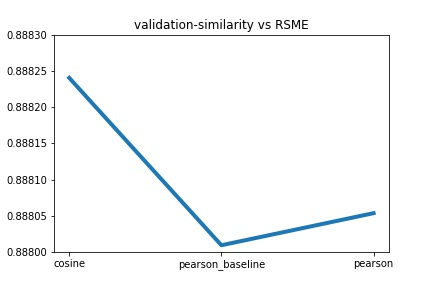
\includegraphics[width=0.30\textwidth]{img/validation-similarity_vs_RSME.jpg}
\label{fig_sim}
\end{figure}

\begin{figure}[H]
\centering
\caption{MAE with different similarity measure}
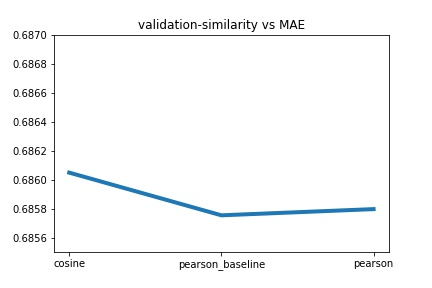
\includegraphics[width=0.30\textwidth]{img/validation-similarity_vs_MAE.jpg}
\label{fig_sim}
\end{figure}


\subsection{Model-Based}
We tested rank from 10 to 50, epochs from 10 to 100, and each parameters from 0.01 to 0.1, and the result is shown in the figure below:
\begin{figure}[H]
\centering
\caption{Tuning Result for NMF model}
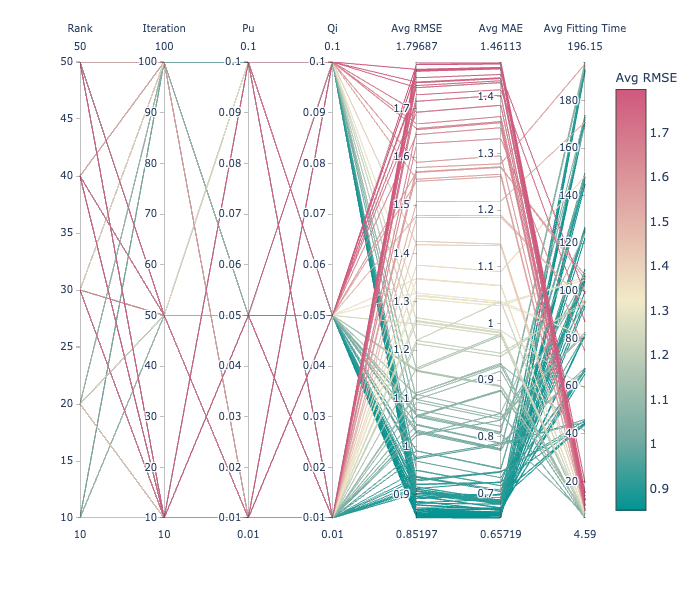
\includegraphics[width=0.45\textwidth]{img/NMF_hypter.png}
\label{fig_sim}
\end{figure}
Since we performed gridsearch on top of cross-validation when searching these parameters, we used parallel coordinate graph to show the results. As the red lines represent bad performance in $RMSE$ and green ones represent better performances, we can see when the models performs worse in $RMSE$ and $MAE$ at a certain combination of parameters. One clear relation we can see is that with more iterations, the result is generally better. Although the other relationships are not as clear, we can observe that lines start from Rank = 50 and Rank = 10 lead to lower RMSE. 

The final model is rank = 50, iteration = 100 with both parameters = 0.1. 


\subsection{Comparison of Results}

We not only explore the performances of the item-based nearest neighbor model and model-based collaborative filtering model, but also compute a baseline model so that we can actually tell whether the performances of our model is good or not. We calculated $RMSE$ and $MAE$ of these three models on the test set, and also the coverage on the test set.

% \begin{table}[H] 
% \centering
% \caption{\label{tab_est:1} RMSE \& MAE Table}
% \label{my-label}
% \begin{tabular}{c|cccccc}
% \hline \hline

% Models          & Split(\%)     & RMSE          &  MAE \\ \hline
% Item-Based      & 80/20         &  0.53508      &  0.78682  \\ \hline
% Item-Based      & 90/10         &  0.37913      &  0.89347  \\ \hline
% Model-Based     & 80/20         &  0.8447       &  0.6571  \\ \hline
% \hline
% \end{tabular}
% \end{table}


\begin{table}[H] 
\centering
\caption{\label{tab_est:1} RMSE \& MAE Table}
\label{my-label}
\begin{tabular}{c|ccccc}
\hline \hline

Models  & RMSE &  MAE  & CC & UC & IC       \\ \hline
Baseline &0.9691 &0.7611 &0.8366 &0.1730 &0.1148 \\ \hline
Item-Based      & 0.8868     &  0.6843   &0.8539 &0.173 &0.09 \\ \hline
Model-Based     &  0.8447       &  0.6571  & 0.8473 & 0.1699 & 0.1309 \\ \hline
\hline
\end{tabular}
\end{table}

Interpretation of results is in the Conclusion section.

\subsection{Further exploration}
To evaluate the model exhaustively, we evaluate the performance of the model not only by tuning the parameters, but also by changing the size of the sample to see how the outputs vary. 

Table 2 and Table demonstrates the evaluation results of two models. We evaluated the running time , $RMSE$, $MAE$, Catalog coverage (CC), User coverage (UC), and Item coverage (IC) when the sample size is 90\% down to 10\% of the train dataset. We changed the size of sample and compared their outputs. As the size of the sample becomes smaller, the running time for both algorithms decreases. We can see that the running time for the nearest-neighbor model increased much faster than the running time of model-based CF as the size increases.

For the item-based method, $RMSE$ varied little for different size, but for model-based method, $RMSE$ increased much more obviously when the size increased. For both methods, we can see that these three coverage rates generally decreased as the size increased. This phenomena is reasonable because as the size increases, more items and users are included in the dataset but we still recommend top-10(at most 10) item to users so the coverage rate could decrease.


% Generally speaking, $RMSE$, $MAE$, CC, UC and IC of our item-based model have value of 0.42, 0.71, 0.89, 0.17, 0.085 respectively. 

\begin{table}[H] 
\centering
\caption{\label{tab_est:1} Item-Based Evaluation Table}
\label{my-label}
\begin{tabular}{c|lccccc}
\hline \hline
Size	    & Time	& RMSE	    & MAE	    & CC	    & UC	    & IC     \\ \hline
0.9         & 442.43	& 0.4209	& 0.6855	& 0.8634	& 0.1703	& 0.0881 \\ \hline
0.8	        & 376.37	& 0.4155	& 0.6875	& 0.8680	& 0.1649	& 0.0901 \\ \hline
0.7	        & 300.52	& 0.4107	& 0.6887	& 0.8799	& 0.1633	& 0.0844 \\ \hline
0.6	        & 225.91	& 0.4064	& 0.6926	& 0.8736	& 0.1629	& 0.0885 \\ \hline
0.5	        & 163.90	& 0.4033	& 0.6965	& 0.8926	& 0.1682	& 0.0873 \\ \hline
0.4	        & 110.61	& 0.4030	& 0.7005	& 0.8903	& 0.1701	& 0.0800 \\ \hline
0.3	        & 73.14	    & 0.4025	& 0.7135	& 0.9086	& 0.1807	& 0.0966 \\ \hline
0.2	        & 43.75	    & 0.4051	& 0.7371	& 0.9311	& 0.1838	& 0.0964 \\ \hline
0.1	        & 23.69	    & 0.4054	& 0.8233	& 0.9729	& 0.1919	& 0.0914 \\ \hline
\hline
\end{tabular}
\end{table}

\begin{table}[H] 
\centering
\caption{\label{tab_est:1} Model-Based Evaluation Table}
\label{my-label}
\begin{tabular}{c|lccccc}
\hline \hline
Size	    & Time	& RMSE	    & MAE	    & CC	    & UC	    & IC     \\ \hline
0.9	        & 61.11	& 0.5854	& 0.6784	& 0.8637	& 0.1671	& 0.0935 \\ \hline
0.8	        & 55.64	& 0.5747	& 0.6800	& 0.8630	& 0.1675	& 0.0938 \\ \hline
0.7	        & 50.34	& 0.5646	& 0.6830	& 0.8668	& 0.1650	& 0.0827 \\ \hline
0.6	        & 45.02	& 0.5483	& 0.6908	& 0.8732	& 0.1635	& 0.0877 \\ \hline
0.5	        & 39.74	& 0.5262	& 0.6977	& 0.8740	& 0.1658	& 0.0846 \\ \hline
0.4	        & 34.80	& 0.4980	& 0.7067	& 0.8886	& 0.1643	& 0.0809 \\ \hline
0.3	        & 29.03	& 0.4521	& 0.7256	& 0.8846	& 0.1704	& 0.0794 \\ \hline
0.2	        & 23.68	& 0.3834	& 0.7536	& 0.9111	& 0.1779	& 0.0855 \\ \hline
0.1	        & 16.54	& 0.2539	& 0.8173	& 0.9565	& 0.2063	& 0.1015 \\ \hline


\hline
\end{tabular}
\end{table}


\begin{figure}[H]
\centering
\caption{Sample Size vs running time}
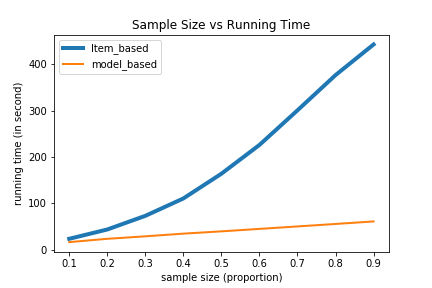
\includegraphics[width=0.30\textwidth]{img/2Svstime.png}
\label{fig_sim}
\end{figure}

\begin{figure}[H]
\centering
\caption{Sample Size vs RMSE}
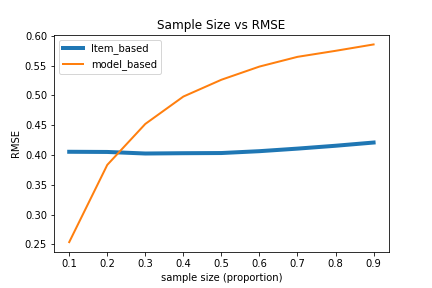
\includegraphics[width=0.30\textwidth]{img/2Svsrmse.png}
\label{fig_sim}
\end{figure}

\begin{figure}[H]
\centering
\caption{Sample Size vs User-coverage}
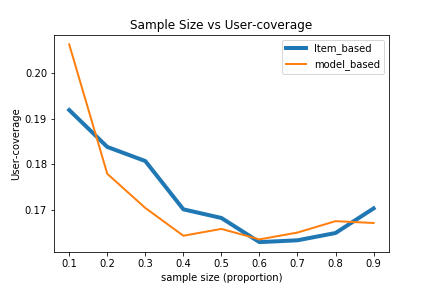
\includegraphics[width=0.30\textwidth]{img/2Svsuc.png}
\label{fig_sim}
\end{figure}

\section{Conclusion}

As our goal is to build a model that predicts the unknown rating of users to movies according to their previous ratings, we carefully evaluated three models and compared their results, $RMSE$, $MAE$, and coverage. From the results section, we can that both item-based mmodel and model-based CF are better than the baseline model in $RMSE$ and $MAE$. And model-based collaborative filtering method has the best performance in $RMSE$ and $MAE$.

Moreover, we can see that IC of item-based model is much lower than IC of model-cased CF. CC and UC of item-based model are slightly better than that of model-cased CF. We can see that one disadvantage of neighborhood methods is their limited coverage caused by sparsity of data.

Compare to model-based CF, neighborhood-based methods are usually simpler and more intuitive to implement and debug. However, in practice, they require more space and longer time to be implemented, as we can see in the experiment of running time vs. scale of dataset, the running time of neighborhood-based method takes much longer than model-based CF. So we can see that model-based recommendation systems require less space and have higher time efficiency. More importantly, they can help in avoiding overfitting. 

It is reasonable that our models and evaluation yield such results that indicate model-based method performs the best.

\section{Future Works}
Due to the limitation of time, we would not able to fully explore other methods and evaluate other metrics. For instance, DCG would also be a good indicator for the performance of the model due to the long tail shape of the distribution of ratings. Since we didn't fully explore other metrics, this could be a potential watch out for the performances of our model. Also, when we recommend movies to users, we only recommend those with high predicted ratings without consider the diversity of the recommendations. Whether diversity would be considered to be important to a recommendation system is decided by whether recommend 'new' items to users is important to that user. This can be solved by analyzing the feedback of the users to our recommended items. We may also perform A/B testing on the ways that we choose to recommend items to users in real world. Further work could be done in the future.

\section{Supplemental Document}
{\bf Code} on GitHub contains developing codes in Jupyter Notebook or Python file format. In this Spark folder in this directory contains the algorithm developed using pyspark. The folder also contains how we did data exploration and plots.

% \ifCLASSOPTIONcaptionsoff
%   \newpage
% \fi
\end{document}